% !TeX spellcheck = en_US
\documentclass[a4paper,9pt]{article}
\usepackage[left=2.5cm, top=2.5cm, right=2.7cm, bottom=2.4cm]{geometry}
\usepackage[utf8]{inputenc}
\usepackage[english]{babel}
\usepackage{multicol}
\usepackage{lmodern}
\usepackage{graphicx}
\usepackage{hyperref}
\usepackage{amsmath}
\usepackage{amsfonts}
\usepackage{pgfplots}
\usepgflibrary{patterns}
\usepgfplotslibrary{fillbetween}
\usepackage{amssymb}
\usepackage{tipa}
\usepackage{mathtools}
\usepackage{fancyvrb}
\usepackage{qtree}
\newcommand{\RA}{$\rightarrow$\ }
\DeclareMathOperator*{\argmax}{arg\,max}
\DeclareMathOperator*{\argmin}{arg\,min}


\newenvironment{uprightmath}
{\changecodes\ignorespaces}
{\ignorespacesafterend}

\newcommand{\changecodes}{%
    \count255=`A
    \loop
    \mathcode\count255=\numexpr\mathcode\count255-\string"100\relax
    \ifnum\count255<`Z
    \advance\count255 1
    \repeat
    \count255=`a
    \loop
    \mathcode\count255=\numexpr\mathcode\count255-\string"100\relax
    \ifnum\count255<`z
    \advance\count255 1
    \repeat
}

\begin{document}
    
    \title{A guide to understand Stepmania's gimmicks}
    \author{
        Pedro G. Bascoy\\
        \texttt{pepo\_gonba@hotmail.com}\\
    }
    \maketitle
   
    \section{From song time to sequencer time}
    \subsection{Stepmania definition}

    The \texttt{SSC} file provides two methods of artificially pausing the note scrolling when the song is playing. Those gimmicks are referred as \texttt{\#STOPS} and \texttt{\#DELAYS}. Although there is a subtle difference between them, they are essentially identical w.r.t. the effect that produces.

One STOP definition might look as follows:

\begin{verbatim}
    #STOPS: 4=5,6=2;
\end{verbatim}

Let us convert the definition into a JSON-like structure:

    \begin{verbatim}
  {
    [
      beat: 4,
      stop: 5 
    ],
    [
      beat: 6,
      stop: 2 
    ]
  }
    \end{verbatim}

    This \texttt{\#STOPS} definition is telling us a couple of things.
    \begin{enumerate}
	    \item At beat 4, stop the scrolling for 5 seconds. Then resume.
	    \item At beat 6, stop the scrolling for 2 seconds. Then resume.
    \end{enumerate}

Similarly, one DELAY defition could look like this:
\begin{verbatim}
    #DELAYS: 4=5,6=2;
\end{verbatim}

And after converting it into the friendly structure:

    \begin{verbatim}
  {
    [
      beat: 4,
      delay: 5 
    ],
    [
      beat: 6,
      delay: 2 
    ]
  }
    \end{verbatim}
    The \texttt{\#DELAYS} definition above is telling us essentially the same story as the STOPS definition shown before, i.e.: 
    \begin{enumerate}
	    \item At beat 4, stop the scrolling for 5 seconds. Then resume.
	    \item At beat 6, stop the scrolling for 2 seconds. Then resume.
    \end{enumerate}

    The difference between these to is that notes that lie exactly at the stop/delay beat, will need to be tapped before and after the waiting time for the stops and delays, respectively.
    \subsection{Challenge}

    We would like to have a function $ t: \mathbb{R} \rightarrow \mathbb{R} $ that would retrieve the song time after stops/delays (sequencer time) from the song time as well as the inverse of this function. Additionally, we would like to have two inverse functions of $ t $, $ t^{-1}_{(s)} $ for STOPS and $ t^{-1}_{(d)} $ for DELAYS.


    \subsection{Solution}

    To do so, let us imagine that we have a function $ f : \mathbb{R}\rightarrow \mathbb{R}$ that given a beat, it calculates the song time. To simplyfy things further, imagine that this song is has constant BPM of 60, so each second is worth 1 beat. Then $ f(b) = b $, being $ b $ a beat.

    Having this in mind, then we can write the piecewise function
    \begin{equation}
	    t(x) = \begin{dcases}
		    x\,, & \text{if $ x \leq f(4) $}\,; \\
		    4\,, & \text{if $4 <  x \leq 4+5 $}\,; \\
		    x-5\,, & \text{if $4 + 5 <  x \leq 6 + 5 $}\,; \\
		    6+5\,, & \text{if $6 + 5 <  x \leq 6 + 5+ 2 $}\,; \\
		    x-2-5\,, & \text{if $ x > 6+5+2 $}\,; \\
	    \end{dcases}
	    \label{l}
    \end{equation}
    that will map from song time to sequencer time. A plot of this function can be see in Figure \ref{fig:songtime2seqtime}. 
    
\begin{figure}[htpb]
	\centering

    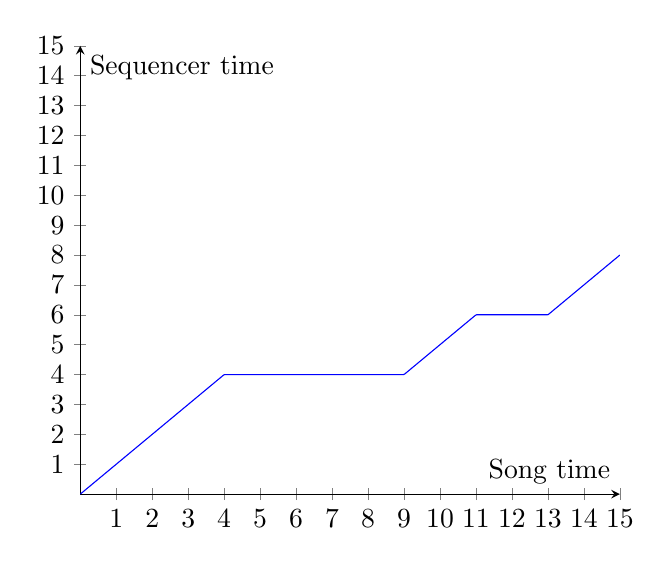
\begin{tikzpicture}[
  declare function={
    func(\x)= (\x<=4) * \x  +
     and(\x>4, \x<=9) * 4  +
     and(\x>9, \x<=11) * (\x-5)  +
     and(\x>11, \x<=13) * (6)  +
     (\x>13) * (\x-7);
  }
]
\begin{axis}[
  axis x line=middle, axis y line=middle,
  ymin=0, ymax=15, ytick={0,...,15}, ylabel=Sequencer time,
  xmin=0, xmax=15, xtick={0,...,15}, xlabel=Song time,
]
\addplot[blue, domain=0:15, samples=400]{func(x)};
\end{axis}
\end{tikzpicture} 
\caption{Plot of $t$ }
	\label{fig:songtime2seqtime}
\end{figure}

    We can calculate the two different inverse functions of $ t(x) $ to model when notes at stops or delays should be tapped w.r.t. the song time. We can write the function

    \begin{equation}
	    t^{-1}_{(s)}(x) =\begin{dcases}
		    x\,, &\text{if $ x \leq 4 $}\,;\\
		    x+5\,,& \text{if $ 4 < x \leq 6 $}\,;\\
		    x+5+2\,,& \text{if $ x > 6 $}\,;\\
	    \end{dcases}
	    \label{eq:tostops}
    \end{equation}
    to map from the sequencer time into song time for STOPS. Similarly, the function

    \begin{equation}
	    t^{-1}_{(d)}(x) =\begin{dcases}
		    x\,, &\text{if $ x < 4 $}\,;\\
		    x+5\,,& \text{if $ 4 \leq x < 6 $}\,;\\
		    x+5+2\,,& \text{if $ x \geq 6 $}\,;\\
	    \end{dcases}
	    \label{eq:todelays}
    \end{equation}
    will map from the sequencer time into the song time for DELAYS. Note that the signs at the conditions are slightly different.


\begin{figure}[htpb]
	\centering

    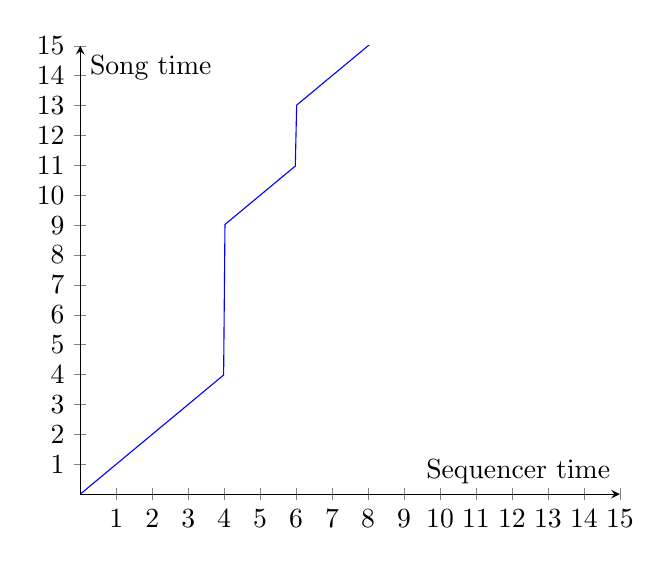
\begin{tikzpicture}[
  declare function={
    func(\x)= (\x<=4) * \x  +
    and(\x>4, \x<=6) * (\x+5)   +
     (\x>6) * (\x+5+2);
  }
]
\begin{axis}[
  axis x line=middle, axis y line=middle,
  ymin=0, ymax=15, ytick={0,...,15}, ylabel=Song time,
  xmin=0, xmax=15, xtick={0,...,15}, xlabel=Sequencer time,
]
\addplot[blue, domain=0:15, samples=400]{func(x)};
\end{axis}
\end{tikzpicture} 

\caption{Plot of $t^{-1}$ }
	\label{fig:seqtime2songtime}
\end{figure}

\subsection{Formalization}


Let $ \mathcal{T} =  \left\{\left( b_i^{(t)}, r_i \right)\right\}_{i=1}^{n} $ be a sequence of STOPS, where $ r_i $ is the stop (measured in seconds) at beat $ b_i^{(t)} $. Let $ f:\mathbb{R}\rightarrow \mathbb{R} $ be a function that retrieves the second from the start of the song given a current beat.

We define a new set 
\begin{equation}
	\mathcal{T'} = \left\{\left( c_i, r_i \right)\right\}_{i=1}^{n} = \left\{\left( f\left( b_i^{(t)}\right), r_i \right)\right\}_{i=1}^{n}
	\label{eq:tprimeset}
\end{equation}
where $ c_i $ is the second from the start of the song of beat $ b_i^{(t)} $.
We define the function $ t: \mathbb{R}\rightarrow \mathbb{R} $
\begin{equation}
	t(x) = \begin{dcases}
		x - \sum_{j=1}^{i-1}r_j\,, & \text{if $ c_{i-1} + \sum_{j=1}^{i-1}r_j < x \leq c_i + \sum_{j=1}^{i-1}r_j\,, \quad \forall i=1,\dots,n$}\,;\\
		c_i\,, & \text{if $ c_i + \sum_{j=1}^{i-1}r_j < x \leq c_i + \sum_{j=1}^i r_j\,,\quad \forall i=1,\dots,n $}\,;\\
		x - \sum_{j=i}^n r_j & \text{if $ x > c_n + \sum_{j=1}^n r_j $}\,; 
	\end{dcases}
	\label{eq:t}
\end{equation}
when $ \mathcal{T'} \neq \emptyset $, where $ c_0 := -\infty $,  that maps from the song time into the sequencer time. 

We define the function $ t_{(s)}^{-1}: \mathbb{R}\rightarrow \mathbb{R} $
\begin{equation}
	t_{(s)}^{-1}(x) = \begin{dcases}
		x\,, & \text{if $ x \leq c_1 $}\,;\\
		x+ \sum_{j=1}^{i}r_i\,, & \text{if $ c_i < x \leq c_{i+1}\,,\quad \forall i=1,\dots,n$}\,;\\
	\end{dcases}
	\label{eq:t-1s}
\end{equation}
with $ c_{i+1} := \infty $ which maps from the sequencer time into the song time for the STOPS, if $ \mathcal{T'} \neq \emptyset $, and the function $ t_{(d)}^{-1}: \mathbb{R}\rightarrow \mathbb{R} $
\begin{equation}
	t_{(d)}^{-1}(x) = \begin{dcases}
		x\,, & \text{if $ x < c_1 $}\,;\\
		x+ \sum_{j=1}^{i}r_i\,, & \text{if $ c_i \leq x < c_{i+1}\,,\quad \forall i=1,\dots,n$}\,;\\
	\end{dcases}
	\label{eq:t-1s}
\end{equation}
that maps from the sequencer time into the song time for the DELAYS, if $ \mathcal{T'}\neq \emptyset $. If $ \mathcal{T'} = \emptyset $, then $ t(x) = t_{(s)}^{-1}(x) = t_{(d)}^{-1} (x) = x $.
    \section{From sequencer time to beat}

    \subsection{Stemania definition}\label{sec:stepmania-definition-time2beat}
    
    A \texttt{SSC} file gives a list of pairs which defines the bpms. The first item in the pair is the target beat, and the second item is the desired BPM from that beat on. Let us imagine we have a \texttt{SSC} file with the following definition:
    \begin{verbatim}
    #BPMS:0,120:8,70:13,200;     
    \end{verbatim}
    Let us convert this cumbersome definition into a friendly structure:
    \begin{verbatim}
  {
    [
      beat: 0,
      bpm: 120
    ],
    [
      beat: 8,
      bpm: 180 
    ],
    [
      beat: 13,
      bpm: 60 
    ]
  }
    \end{verbatim}

    This \texttt{\#BPMS} definition is telling us three things:
    \begin{enumerate}
	    \item From beat $- \infty$ to beat 8, the BPM is 120.
	    \item From beat 8 to beat 13, the BPM is 180.
	    \item From beat 13 to beat $+\infty$, the BPM is 60.
    \end{enumerate}

    \subsection{Challenge}

    We want to find a function $f : \mathbb{R} \rightarrow \mathbb{R}$ that retrieves the current beat given the second.  This function is useful when a song is playing and we want to know at what beat we are at if we know how much time has passed since the start of the song. Notes move at the speed of the BPM, so if we can have a function $f$, we can sort of know where the steps should be drawn.

    \subsection{Solution}

    First, let us convert BPMS to BPSS (Beats Per Second), since we are going to provide the input in seconds instead of minutes. We can do so by dividing the BPMS by 60, i.e.
    \begin{equation}
	    \text{BPS}(x) = x \times \frac{\text{Beats}}{\text{Minute}} = x \times \frac{1 \times \text{Minute}}{60 \times \text{Seconds}} \frac{\text{Beats}}{\text{Minute}} = \frac{x}{60} \times \frac{\text{Beats}}{\text{Second}}\,. 
	    \label{eq:bpm2bps}
    \end{equation}

    Next, let us define a piecewise function $f': \mathbb{R} \rightarrow \mathbb{R}$ that gives the current BPS given the current Beat. Taking the \texttt{\#BPMS} toy example from the previous section, we get that
    \begin{equation}
	    f'(x) = \begin{dcases}
		    2\,, & \text{if $x \leq 8\,;$}\\ 
		    3\,, & \text{if $8 < x \leq 13\,;$}\\ 
		    1\,, & \text{if $x > 13\,.$}\\ 
	    \end{dcases}
	    \label{eq:beat2bps}
    \end{equation}

    In Figure \ref{fig:beat2bps} you can see the plot of $f'$ we just defined in \eqref{eq:beat2bps}. 

\begin{figure}[htpb]
	\centering

    \begin{tikzpicture}[
  declare function={
    func(\x)= (\x<=8) * 2  +
     and(\x>8, \x<=13) * 3  +
     (\x>13) * (1);
  }
]
\begin{axis}[
  axis x line=middle, axis y line=middle,
  ymin=0, ymax=5, ytick={0,...,5}, ylabel=BPS,
  xmin=0, xmax=15, xtick={0,...,15}, xlabel=Beat,
]
\addplot[blue, domain=0:15, samples=400]{func(x)};
\end{axis}
\end{tikzpicture} 


	\caption{Plot of $f'$}
	\label{fig:beat2bps}
\end{figure}

Note that by using $f'$, we can get the BPS at any beat of the song. This is great, but it does not quite solve our problem. 

Next, we can calculate the SPB (Seconds Per Beat) by just inversing the BPS, i.e.
\begin{equation}
	\text{SPB} = \frac{1}{\text{BPS}}\,,
	\label{eq:bps2spb}
\end{equation}
and therefore we can define a function $t: \mathbb{R} \rightarrow \mathbb{R}$

\begin{equation}
	t(x) = x\times \text{SPB}
	\label{eq:beat2seconds}
\end{equation}
that given a beat $x$ retrieves the current second.

Let 



    \begin{equation}
	    f''(x) = \begin{dcases}
		    \frac{x}{2}\,, & \text{if $x \leq 8\,;$}\\[1em]
		    \frac{8}{2}+\frac{x-8}{3}\,, & \text{if $8 < x \leq 13\,;$}\\[1em]  
		    \frac{8}{2}+\frac{5}{3}+x- 13\,, & \text{if $x > 13\,;$}\\ 
	    \end{dcases}
	    \label{eq:beat2second}
    \end{equation}
    be the function that given a beat $x$ retrieves the current second. This function is the result of plugging \eqref{eq:bps2spb} and \eqref{eq:beat2seconds} into \eqref{eq:beat2bps}, and can be rewritten recursively as

    \begin{equation}
	    f''(x) = \begin{dcases}
		    \frac{x}{2}\,, & \text{if $x \leq 8\,;$}\\[1em]
		    f''(8)+\frac{x-8}{3}\,, & \text{if $8 < x \leq 13\,;$}\\[1em]  
		    f''(13) + x- 13\,, & \text{if $x > 13\,.$}\\ 
	    \end{dcases}
	    \label{eq:beat2second}
    \end{equation}

    Figure \ref{fig:beat2second} depicts the function $f''$. Note that this is just the opposite of the desired solution!
    
\begin{figure}[htpb]
	\centering

    \begin{tikzpicture}[
  declare function={
	  func(\x)= (\x<=8) * (\x/2)  +
	  and(\x>8, \x<=13) * (8/2 + (\x-8)/3)  +
     (\x>13) * (8/2 + 5/3 +\x - 13);
  }
]
\begin{axis}[
  axis x line=middle, axis y line=middle,
  ymin=0, ymax=9, ytick={0,...,9}, ylabel=Second,
  xmin=0, xmax=15, xtick={0,...,15}, xlabel=Beat,
]
\addplot[blue, domain=0:15, samples=400]{func(x)};
\end{axis}
\end{tikzpicture} 
	\caption{Plot of $f''$}
	\label{fig:beat2second}
\end{figure}

As it turns out, the function $f$ that we are looking for is just the inverse function of $f''$, in short
\begin{equation}
	f = f''^{-1}\,,
	\label{eq:inverse}
\end{equation}

thus

    \begin{equation}
    f(x) = \begin{dcases}
		    2x\,, & \text{if $x \leq 4\,;$}\\[1em]
		    (x-4)\times 3 + 8\,, & \text{if $4 < x \leq 5.6\,;$}\\[1em]  
		    x-5.6 + 13\,, & \text{if $x > 5.6\,.$}\\ 
	    \end{dcases}
	    \label{eq:beat2second}
    \end{equation}
    
    A plot of $f$ can be seen in Figure \ref{fig:second2beat}.
\begin{figure}[htpb]
	\centering

    \begin{tikzpicture}[
  declare function={
	  func(\x)= (\x<=4) * (2*\x)  +
	  and(\x>4, \x<=5.66666) * (3*(\x-4)+8)  +
	  (\x>5.66666) * ((\x-5.66666) + 13);
  }
]
\begin{axis}[
  axis x line=middle, axis y line=middle,
  ymin=0, ymax=15, ytick={0,...,15}, ylabel=Beat,
  xmin=0, xmax=9, xtick={0,...,9}, xlabel=Second,
]
\addplot[blue, domain=0:9, samples=400]{func(x)};
\end{axis}
\end{tikzpicture} 
	\caption{Plot of $f$}
	\label{fig:second2beat}
\end{figure}

\subsection{Formalization}
Let $d = \{\left( b_i, v_i \right)\}_{i=1}^{n}$ be a sequence of $n$ beat signatures, where $v_i$ is the BPS  value at beat $b_i$. 
Let $ f: \mathbb{R} \rightarrow \mathbb{R} $ be a function that provided a beat, returns the seconds from the first beat. We define this function as a $n$-step piecewise function
    \begin{equation}
	    f(x) = \begin{dcases}
		    \frac{x}{v_1}\,, & \text{if $x \leq b_{2} $ }\,;\\
		    f(b_{i}) + \frac{x-b_{i}}{v_i}\,, & \text{if $b_{i} < x \leq b_{i+1}\,; \quad \forall i=2,\ldots,n $}\,; \\
	    \end{dcases}
	    \label{eq:beat2second}
    \end{equation}
    where $ b_1 := 0$,  and $b_{n+1} := \infty$.
    
    Analogously, let $ g: \mathbb{R} \rightarrow \mathbb{R} $ be a function that provided a second, returns the beat from the zero second. We define this function as a $n$-step piecewise function
    \begin{equation}
	    g(x) = \begin{dcases}
		    v_1x\,, & \text{if $x \leq f(b_{2}) $ }\,;\\
		    \left[x-f(b_{i})\right]\times v_i + b_{i}\,, & \text{if $f(b_{i}) < x \leq f(b_{i+1})\,;\quad \forall i=2,\ldots,n$}\,, \\
	    \end{dcases}
	    \label{eq:beat2second}
    \end{equation}
    where $g = f^{-1}$.

    \section{From beat to note position}

    \subsection{Stepmania definition}

    There are a pair of stepmania definitions that influence the position where notes should be placed on the screen. One of them is \texttt{\#BPMS}, which arguably is the rate at what notes travel upwards towards the receptor w.r.t. to the music rhythm. As well see later on, we will consider the BPMS as a speed function from which we can discover the position of a note given the beat it should be tapped. As a toy example, we will use the same definition as provided in Section \ref{sec:stepmania-definition-time2beat}. 

    However, there is another gimmick that plays a role in the note positioning: \texttt{\#SCROLLS}. Let's have a look at an example:

    \begin{verbatim}
    #SCROLLS:0=1,4=0,10=2;     
    \end{verbatim}
    Again, let us convert this cumbersome definition into a friendly structure:
    \begin{verbatim}
  {
    [
      beat: 0,
      scroll: 1
    ],
    [
      beat: 4,
      scroll: 0 
    ],
    [
      beat: 10,
      scroll: 2 
    ]
  }
    \end{verbatim}
    The scroll gimmick changes the effective BPM at a given beat by a rate defined by the scroll value. Thus, in this example, the SCROLLS gimmick is changing the BPMs as follows:
    \begin{enumerate}
		\item From beat 0 to beat 4, the BPM is its value times 1.
		\item From beat 4 to beat 10, the BPM is its value times 0. (all the steps in between this beats, will have the same position)
		\item From beat 10 on, the BPM is its value times 2.
    \end{enumerate}
    \subsection{Challenge}

    We would like to have a function $ p: \mathbb{R} \rightarrow \mathbb{R} $ that given a beat, it retrieves the position w.r.t. the origin (or where the receptor is) where a note at that beat should be drawn.

    \subsection{Solution}
    Let us start by defining a function $h: \mathbb{R} \rightarrow \mathbb{R}$ that retrieves the current BPS (Beats per Second) from the current beat. Given the example, this function is identical to that of \eqref{eq:beat2bps},

    \begin{equation}
	    h(x) = \begin{dcases}
		    2\,, & \text{if $x \leq 8\,;$}\\ 
		    3\,, & \text{if $8 < x \leq 13\,;$}\\ 
		    1\,, & \text{if $x > 13\,.$}\\ 
	    \end{dcases}
	    \label{eq:beat2bps-as-h}
    \end{equation}

    You can see a plot of this function in Figure  \ref{fig:beat2bps}. Now, let us define a new function $g: \mathbb{R}\rightarrow \mathbb{R}$ that given a beat, retrieves the effective BPS (i.e., BPS with applied scrolls). For that matter, we just need to check out in what beats the scroll is taking place, and change the BPS accordingly. For our toy example the resultant $g$ function looks like this
    \begin{equation}
	    g(x) = \begin{dcases}
		    1\times 2\,, & \text{if $x \leq 4\,;$}\\ 
		    0\times 2\,, & \text{if $4 < x \leq 8\,;$}\\ 
		    0\times 3\,, & \text{if $8 < x \leq 10\,;$}\\ 
		    2\times 3\,, & \text{if $10 < x \leq 13\,;$}\\ 
		    2\times 1 \,, & \text{if $x > 13\,.$}\\ 
	    \end{dcases}
	    \label{eq:beat2effective-bps}
    \end{equation}

    The function $g$ is depicted in Figure \ref{fig:beat2effective-bps}.
\begin{figure}[htpb]
	\centering

    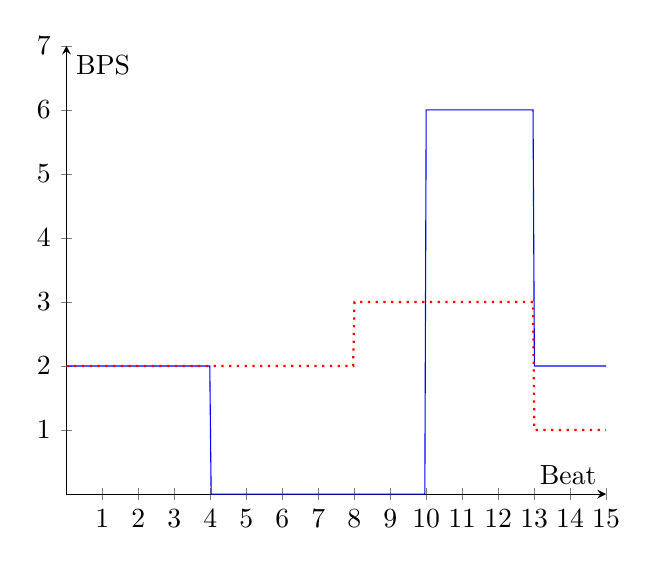
\begin{tikzpicture}[
  declare function={
    func(\x)= (\x<=4) * 2  +
     and(\x>4, \x<=8) * 0  +
     and(\x>8, \x<=10) * 0  +
     and(\x>10, \x<=13) * 6 +
     (\x>13) * (2);
  },
  declare function={
    func2(\x)= (\x<=8) * 2  +
     and(\x>8, \x<=13) * 3  +
     (\x>13) * (1);
  }
]
\begin{axis}[
  axis x line=middle, axis y line=middle,
  ymin=0, ymax=7, ytick={0,...,7}, ylabel=BPS,
  xmin=0, xmax=15, xtick={0,...,15}, xlabel=Beat,
]
\addplot[blue, domain=0:15, samples=400]{func(x)};
\addplot[red, dotted, thick, domain=0:15, samples=400]{func2(x)};
\end{axis}
\end{tikzpicture} 
\caption{Plot of $g$ (blue line), Plot of $h$ (dotted, red line)}
	\label{fig:beat2effective-bps}
\end{figure}
Now, this is great! By asking $g$, now we have the effective BPS. Note that $g$ is a function that models speed, i.e. the velocity that the notes should move towards the receptor.
To retrieve the position at each beat, we can just consider that $\frac{dp}{dx} = g(x)$. Therefore, to get $p$, we just have to take in integral of $g$ w.r.t. $x$,
\begin{equation}
p(x) = \int g(x) dx\,.
	\label{eq:beat2position}
\end{equation}

For instance, if we want to know the position of a note at the beat 11, it would only take to calculate 
\begin{equation}
	\text{position} = \int_{0}^{11} g(x) dx\,.
	\label{eq:beat2position-example}
\end{equation}

You can see an example in Figure \ref{fig:example-area}. As shown, the position  at beat 11 is the area under the curve (in light blue) from 0 to 11.

\begin{figure}[htpb]
	\centering

    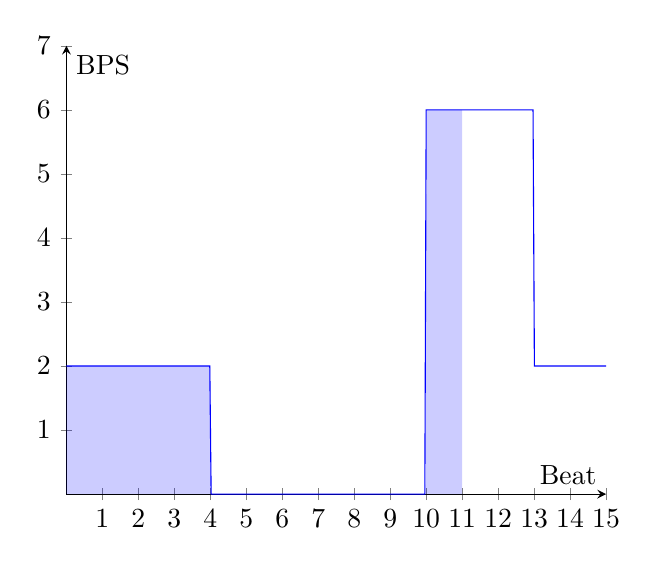
\begin{tikzpicture}[
  declare function={
    func(\x)= (\x<=4) * 2  +
     and(\x>4, \x<=8) * 0  +
     and(\x>8, \x<=10) * 0  +
     and(\x>10, \x<=13) * 6 +
     (\x>13) * (2);
  }
]
\begin{axis}[
  axis x line=middle, axis y line=middle,
  ymin=0, ymax=7, ytick={0,...,7}, ylabel=BPS,
  xmin=0, xmax=15, xtick={0,...,15}, xlabel=Beat,
]
\addplot[blue, domain=0:15, samples=400]{func(x)};
\addplot[draw=none,blue, domain=0:11, samples=400, name path=A]{func(x)};
\addplot[draw=none,name path=B, domain=0:11] {0};
\addplot+[blue, fill opacity=0.2] fill between[of=A and B, soft clip={domain=0:15}];
\end{axis}
\end{tikzpicture} 
\caption{The position at beat 11 will be the area underneeth the function $g$.}
	\label{fig:example-area}
\end{figure}
The resulting integral of $g(x)$ in our toy example is
    \begin{equation}
	    p(x) = \begin{dcases}
		    2x\,, & \text{if $x \leq 4\,;$}\\ 
		    p(4) + 0\,, & \text{if $4 < x \leq 8\,;$}\\ 
		    p(8) + 0\,, & \text{if $8 < x \leq 10\,;$}\\ 
		    p(10) + (x-10)\times6 \,, & \text{if $10 < x \leq 13\,;$}\\ 
		    p(13) + (x-13) \times 1 \,, & \text{if $x > 13\,,$}\\ 
	    \end{dcases}
	    \label{eq:beat2effective-bps}
    \end{equation}
    and its plot can be seen in Figure \ref{fig:position-example}.


\begin{figure}[htpb]
	\centering
    \begin{tikzpicture}[
  declare function={
	  func(\x)= (\x<=4) * (2*\x)  +
	  and(\x>4, \x<=8) * (8)  +
     and(\x>8, \x<=10) * 8  +
     and(\x>10, \x<=13) * (8 + (\x-10)*6) +
     (\x>13) * (26 + (\x-13)*2);
  }
]
\begin{axis}[
  axis x line=middle, axis y line=middle,
  ymin=0, ymax=30, ytick={0,5,...,30}, ylabel=Position,
  xmin=0, xmax=15, xtick={0,...,15}, xlabel=Beat,
]
\addplot[blue, domain=0:15, samples=400]{func(x)};
\end{axis}
\end{tikzpicture} 
\caption{Plot of $ p $}
	\label{fig:position-example}
\end{figure}
    \subsection{Formalization}

    Let
    \begin{equation}
	    \left\{\left( b_{i}^{(b)},v_{i} \right)\right\}_{i=1}^{n} = \mathcal{B} = B^{(b)} \times V
	    \label{eq:B}
    \end{equation}
    be a sequence of $n$ beat signatures, where $v_i \in V = \{v_j\}_{j=1}^{n}$ is the BPS value at beat $b_i^{(b)} \in B^{(b)} = \{b_i^{(b)}\}_{j=1}^{n}$.

    Let

    \begin{equation}
	    \left\{ \left( b_{i}^{(s)},s_{i} \right) \right\} _{i=1}^{m} = \mathcal{S} = B^{(s)} \times S
	    \label{eq:S}
    \end{equation}
    be a sequence of $m$ scroll signatures, where $s_i \in S = \{s_j\}_{j=1}^{m}$ is the scroll value at beat $b_i^{(s)} \in B^{(s)}= \{b_j^{(s)}\}_{j=1}^{m}$.

 Let  
    \begin{equation}
	    \left\{ \left( b_{i},z_{i} \right) \right\} _{i=1}^{n'} = \mathcal{Z} = B^{(b)} \cup B^{(s)}\times V \cup S
	    \label{eq:Z}
    \end{equation}
    be a sequence of $n'$ BPSs with applied scrolls, where $z_i$ is the effective BPS at beat $b_i$
    constructed from $\mathcal{S}$ and $\mathcal{B}$ as 
    \begin{equation}
	    \mathcal{Z} = \bigcup_{i=1}^{m} \left\{\left( b_i^{(s)},h(b_i^{(s)})\times s_i \right)\right\}\bigcup_{j=1}^{n} 
	    \begin{dcases}
		    \left\{ \left( b_j^{(b)}, v_j\times s_i \right)\right\}\,, & \text{if $b_i^{(s)} < b_j^{(b)} < b_{i+1}^{(s)}$}\,; \\
		    \emptyset\,, & \text{otherwise}\,;
	    \end{dcases}
	    \label{eq:Z-construction}
    \end{equation}
    where $h: \mathbb{R} \rightarrow \mathbb{R}$ is a function that given a beat, returns the BPS for that beat, and $b_{m+1}^{(s)} := \infty$.
    We define
    \begin{equation}
	    g(x) = \begin{dcases}
		    z_1\,, & \text{if $ x \leq b_2 $}\,;\\
		    z_i\,, & \text{if $ b_{i} < x \leq b_{i+1}\,; \quad \forall i=2,\dots,n'$}\,,
	    \end{dcases}
	    \label{eq:final-g}
    \end{equation}
    as a function that retrieves the effective BPS given a beat, and $ b_{n'+1}:= \infty $. Finally, we define 
    \begin{equation}
	    p(x) = \int g(x) dx = \begin{dcases}
		    xz_1\,, & \text{if $ x \leq b_2 $}\,;\\
		    p(b_i) + (x-b_i)\times z_i\,, & \text{if $ b_{i} < x \leq b_{i+1}\,; \quad \forall i=2,\dots,n'$}\,,
	    \end{dcases}
	    \label{eq:position-final}
    \end{equation}
    as the function that retrieves the position given a beat.

\end{document}



